\documentclass[12pt]{article}
\usepackage[utf8]{inputenc}
\usepackage[english]{babel}
\usepackage{listings}
\usepackage{tikz}
\usepackage{amsmath,amssymb}
\usepackage{subcaption}

\newcommand{\HRule}{\rule{\linewidth}{0.5mm}}

% Listings
\newlength{\eightytt}
\newcommand{\testthewidth}{%
  \fontsize{\dimen0}{0}\selectfont
  \sbox0{x\global\dimen1=0.6em}%
  \ifdim \dimexpr80\dimen1+23pt>\textwidth
    \advance\dimen0 by -.1pt
    \expandafter\testthewidth
  \else
    \global\eightytt\dimen0
  \fi
}
\AtBeginDocument{%
  \dimen0=\csname f@size\endcsname pt
  \begingroup
  \ttfamily
  \testthewidth
  \endgroup
  \lstset{
    % columns=fullflexible,
    basicstyle=\fontsize{\eightytt}{1.2\eightytt}\ttfamily
               \color[HTML]{F8F8F2},
    breaklines=true
  }
}
\lstset{
  breaklines=true,
  backgroundcolor=\color[HTML]{282828},
  framexleftmargin=2pt,
  inputencoding=utf8,
  captionpos=b,
  numbers=none,
  numberstyle = \fontsize{\eightytt}{1.2\eightytt}
                \color[HTML]{282828},
  keywordstyle =    \color[HTML]{F92672}\ttfamily,
  commentstyle =    \color[HTML]{75715E}\ttfamily,
  stringstyle =     \color[HTML]{E6DB74}\ttfamily,
  % identifierstyle = \color[HTML]{F8F8F2}\ttfamily,
  showstringspaces=false
}
\lstdefinestyle{compact} {aboveskip={0.1\baselineskip}}
\lstdefinestyle{notcompact} {aboveskip={1.2\baselineskip}}
\lstdefinestyle{numbered} {numbers=left,xleftmargin=0pt}
\lstdefinestyle{appendix} {backgroundcolor=\color{white}}
%%%% End listings

\begin{document}

\begin{center}
\textsc{\LARGE Principles of Computer System Design}\\[0.3cm] % Context
\HRule \\[0.4cm]
{ \huge \bfseries Assignment 4}
\HRule \\[0.4cm]
\large
Johannes de Fine Licht
\\Philip Graae
\\Ola Rønning
\\\today
\end{center}

\section*{Question 1: Reliability}

The two networks discussed below are shown in figure~\ref{fig:networks}.

\subsection*{1.}

For the daisy chain to connect all the buildings, both links must be active. Links have the probability of failing $p$, resulting in the added probability of failure $p_\text{daisy} = p + p - p\cdot p = 2p - p^2$. So the probability of the buildings being connected is $P(connected) = 1 - (2p - p^2)$

\subsection*{2.}


For the fully connected network to fail, any two links would have to fail. This is the probability that any two links fail added to the probability that all 3 links fail. The probability of all 3 links failing is $P(ABC) = p^{3}$. The probability of 2 links failing is (say for A and B failing) $P(A\cap B) = p^{2}\cdot(1-p)$, because it is the probability of 2 links failing AND one link not failing (hence $1-p$). Since this can happen in 3 different ways, each with equal probability, the probability for 2 links failing is $P(AB \cup AC \cup BC) = 3p^2 - 3p^3$, and this added with the probability for all 3 failing leaves $P(AB \cup AC \cup BC \cup ABC) = 3p^2 - 2p^3$. So the probability that all the buildings are connected is just $P(connected) = 1 - (3p^2 - 2p^3)$.

% For the fully connected network to fail, any two links would have to fail. This is the probability that any one link of the three links will fail, followed by the probability that any one of the remaining two links will fail. The event of a link failing is denoted as $A$, $B$ and $C$ in the below:
%
% \begin{align*}
%   P(((A\cup B)\cup C)\cap (A\cup B)) = ((P(A) + P(B) - P(A\cap B)) \\
%   \cap P(C)) \cup (P(A) + P(B) - P(A\cap B)) \\
%   = (P(A) + P(B) - P(A\cap B) + P(C) + P(C) \cap (P(A) + P(B) - P(A\cap B))) \\
%   \cap (P(A) + P(B) - P(A\cap B)) \\ \Rightarrow
%   p_{\text{full}} = (p + p - p^2 + p + p\cdot(p + p - p^2)) \cdot (p + p - p^2)\\
%   = p^5 - 3p^4 - p^3 + 6p^2
% \end{align*}


\subsection*{3.}

Probabilities of failure for the networks are now $p_{\text{daisy}} = 10^{-6}$ and $p_{\text{full}} = 10^{-4}$. \\
Based on the expressions derived above, this results in the probabilities:

\begin{align*}
  p_{\text{daisy}} = 2\cdot10^{-6} - 10^{-6\cdot2} \approx 2\cdot10^{-6} \\
  p_{\text{full}} = 3(10^{-4})^2 - 2(10^{-4})^3 \approx 3\cdot10^{-8}
\end{align*}

Even though the probability of a single link failing in the daisy network as compared to the full network is a hundred times lower, the more failure-tolerant design of the full network makes it the most reliable.

\subsection*{Assumptions}

In the above it has been assumed that:
\begin{itemize}
  \item Failures of different links are uncorrelated. In real-world scenarios, the source of a failure can often affect multiple components (lacking dissipation of heat, power outage, meteor strikes).
  \item The probability of $p$ is a \emph{probability of failure per unit of measurement}, where the unit of measurement can be a metric such as time or iterations. In the above the probability is assumed to be constant, while in normal hardware, the probability of failure typically is not constant in time/iterations.
  \item For the fully connected network, the probability is calculated from the assumption that the two (or three) failures happen within the same measurement. That is, if we measure the system and observe 1 link being down, we have to reset the system (fix the link) for the probability to hold for the next measurement.
\end{itemize}

\begin{figure}
\begin{subfigure}{.5\textwidth}
\centering
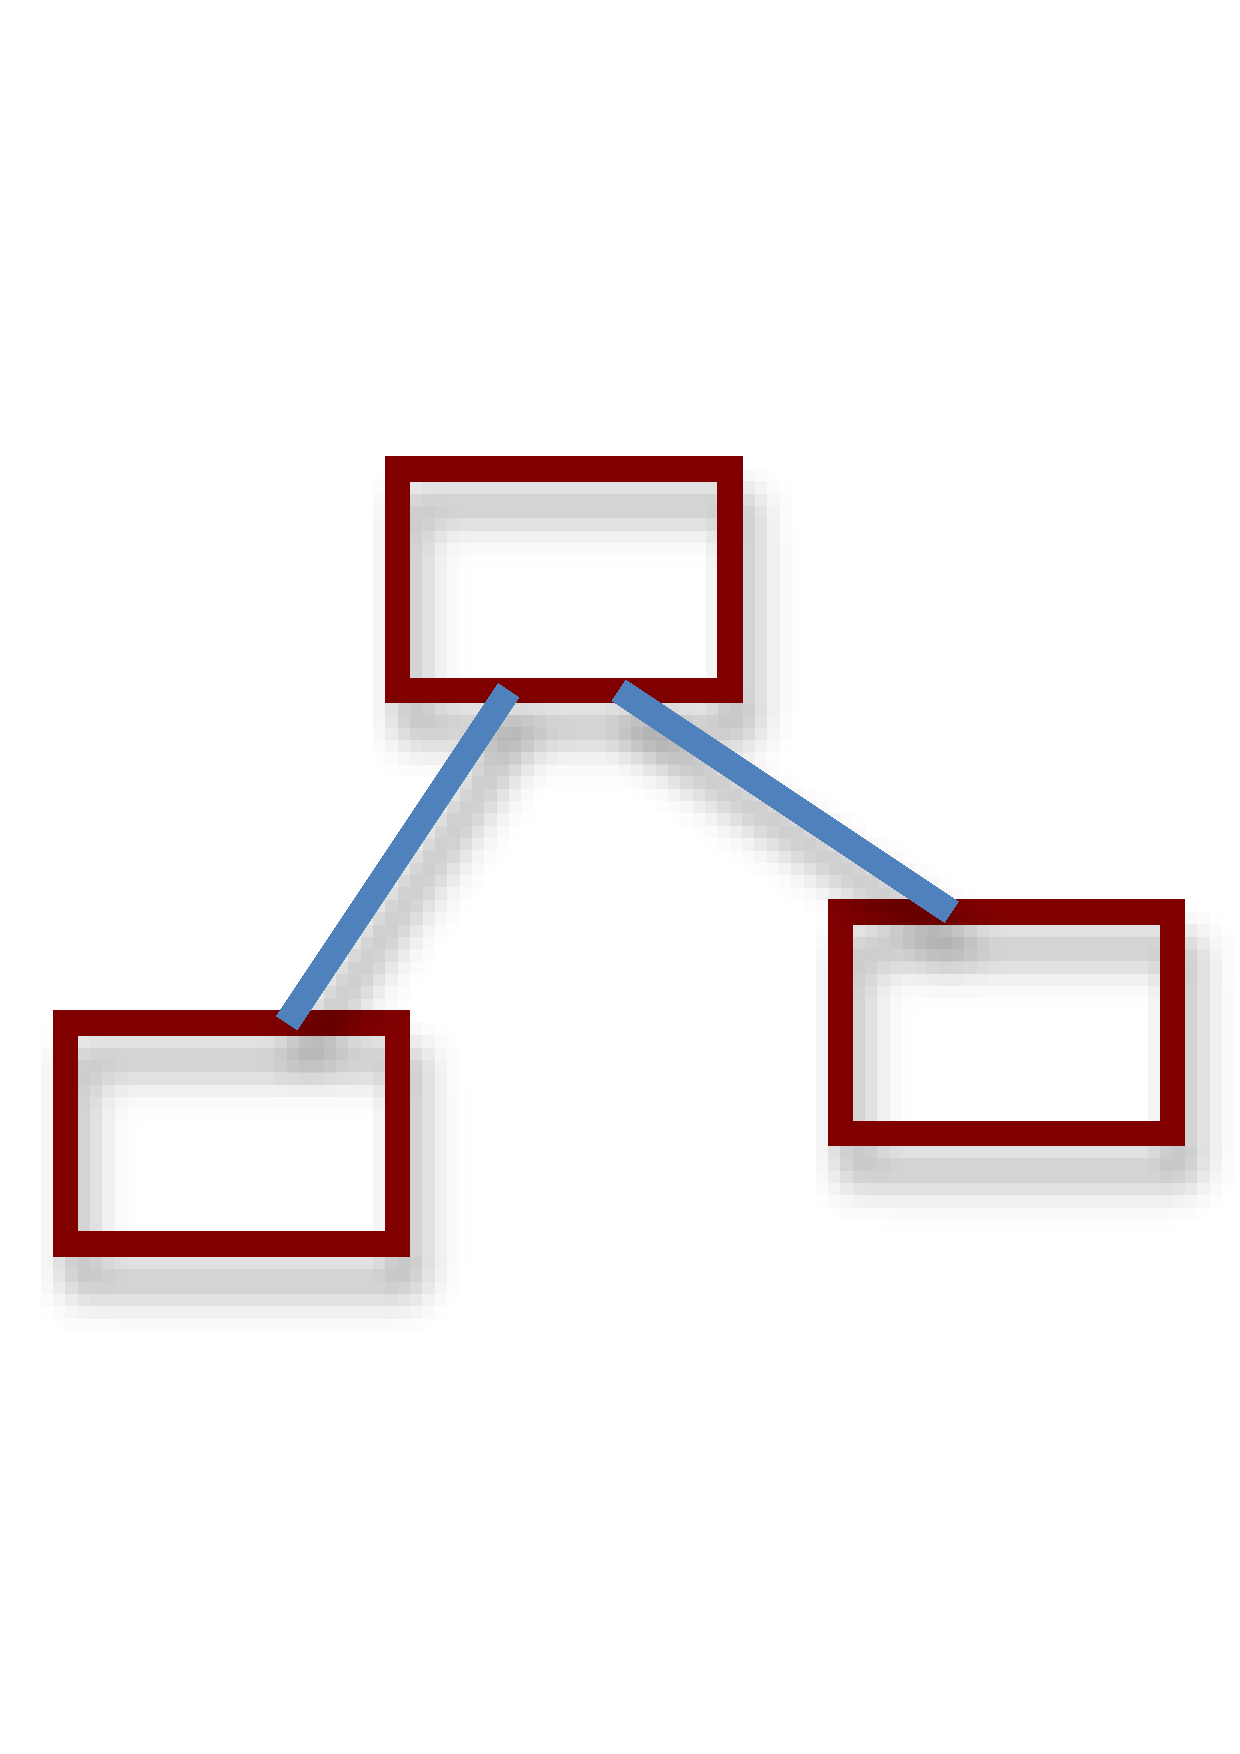
\includegraphics[width=.5\textwidth]{daisychain.pdf}
\caption{Daisy chain network.}
\end{subfigure}
\begin{subfigure}{0.5\textwidth}
\centering
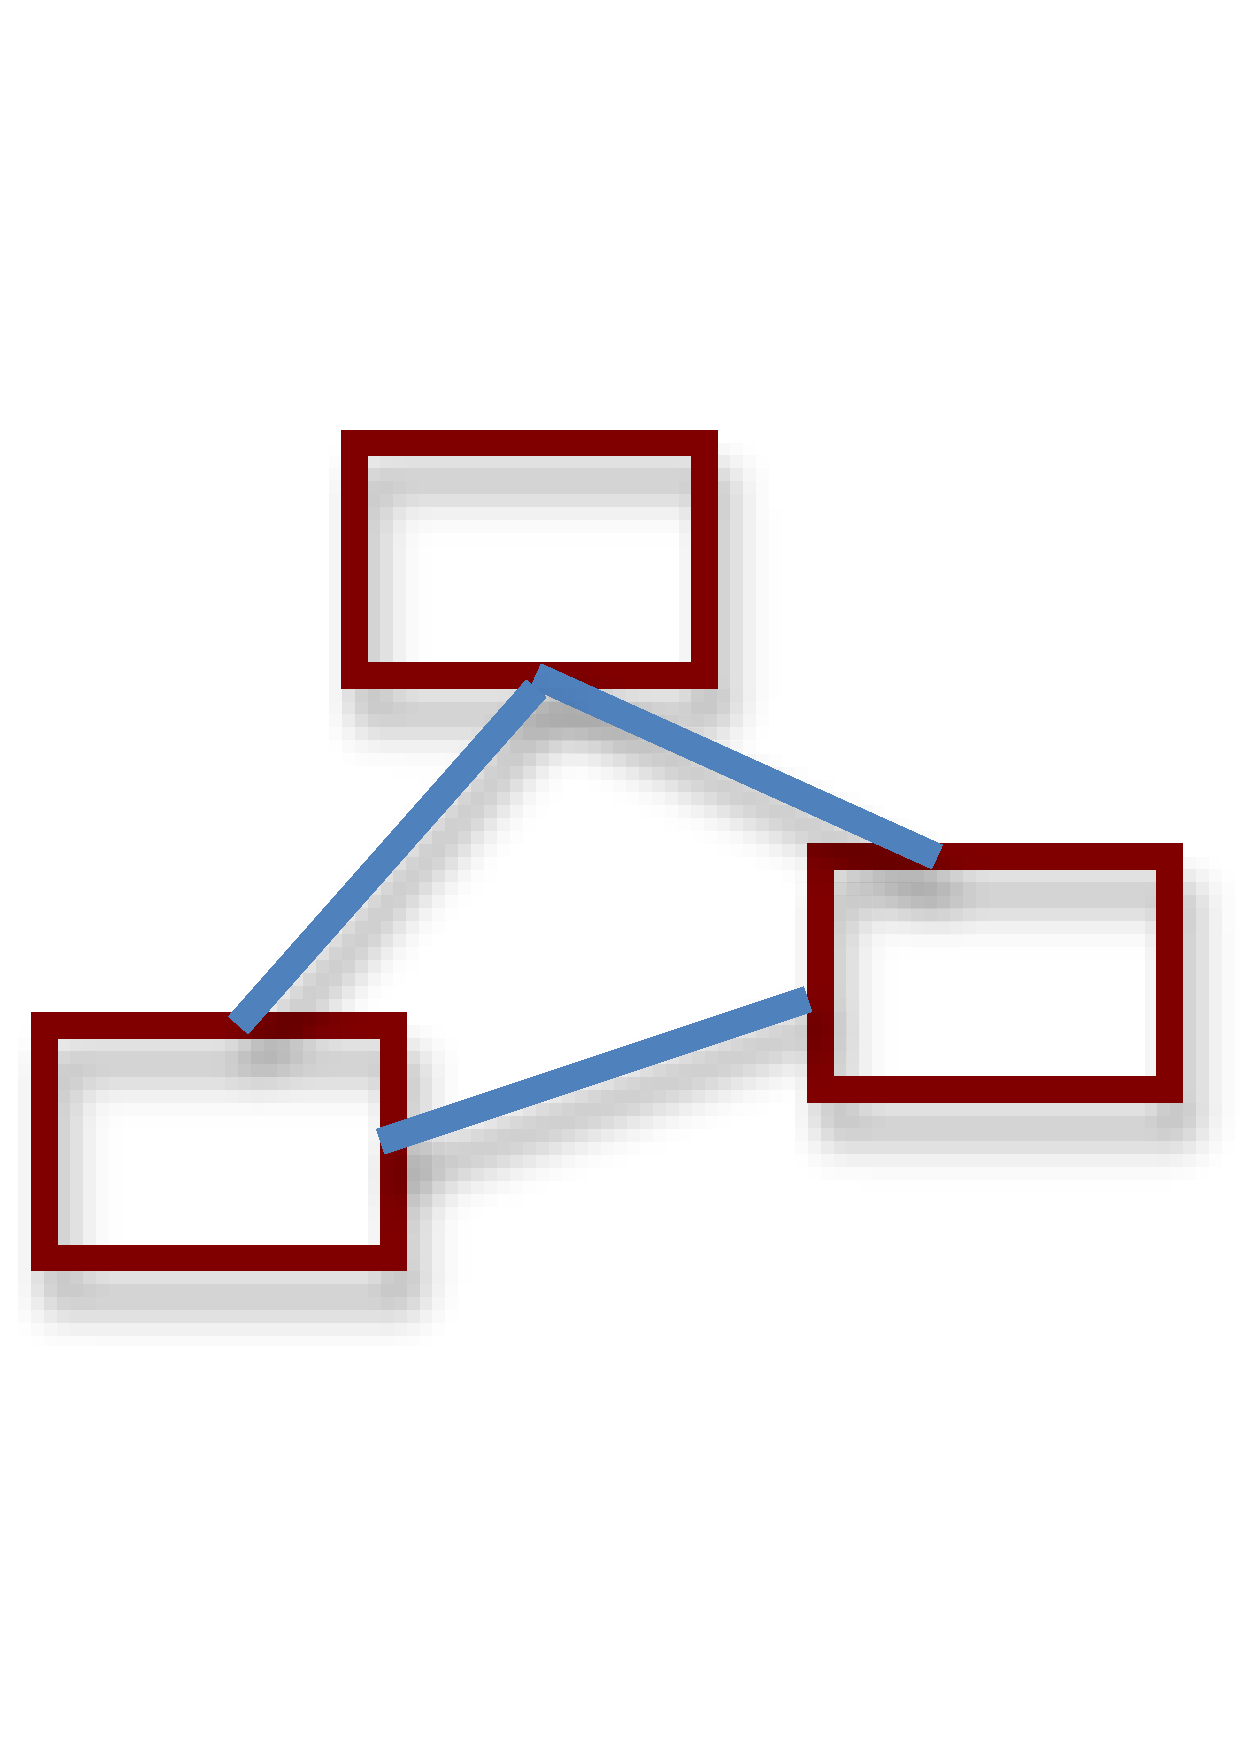
\includegraphics[width=.5\textwidth]{fullyconnected.pdf}
\caption{Fully connected network.}
\end{subfigure}
\caption{The two network models described in Question 1.}
\label{fig:networks}
\end{figure}

\section*{Question 2: Distributed Coordination}

For a two phase commit protocol, there is a risk of indefinite blocking if the coordinator and a participant both experience failure. This can occur after the voting phase, as the other nodes will not know whether the coordinator had already sent a commit or abort message to the crashed participant, and as such cannot proceed before receiving communication from the failed nodes. \\
For the three phase commit, the nodes first enter a \emph{preCommit} stage, then notify the coordinator that they are ready to commit. The coordinator will wait for acknowledgements from all nodes before sending the \emph{doCommit} message. If the coordinator and a participant fail at this stage, the other nodes will know and agree that both failed nodes were ready and had acknowledged the commit, resolving ambiguity concerning the state of the system which would otherwise requiring blocking following a two phase commit protocol.

\section*{Questions for Discussion on the Replication mechanism}

\subsection*{1.}
\subsubsection*{Replication interface}
A new interface \verb|Replication| is added with the single method signature:
\begin{lstlisting}[language=Java]
public ReplicationResult replicate(ReplicationRequest request);
\end{lstlisting}
\subsubsection*{Replication client side proxy}
A new class \verb|ReplicationHTTPProxy| is added as a master bookstore-level HTTP proxy to interacting with slaves. It implements the \verb|Replication| interface as the client side.
\subsubsection*{Replicator and replication tasks}
During initialization, the master bookstore will pass the list of slave server addresses to the \verb|CertainBookStoreReplicator| class during construction. The replicator will then instantiate a \verb|ReplicationHTTPProxy| for each slave in the list. When a replication request is made, the replicator promises a future \verb|CertainBookStoreReplicationTask| for each slave, drawn from a fixed size thread pool implementing Java's \verb|ExecutorService| interface. \\
Each replication task receives an object implementing \verb|Replication| in its constructor along with the request, on which it runs \verb|replicate| with the request when called. In this way it is decoupled with the communication model.
\subsubsection*{Server side replication}
The message handler of the slave servers is extended to handle replication messages. The content of the replication will simply be executed on the underlying bookstore server, returning whether the operation has succeeded.
\subsubsection*{Load balancing}
Instead of the suggested \verb|getReplicaAddress| method, an alternative method \verb|getLowestWorkload| is used. Each of the client proxies maintains a list of \verb|ServerWorkload| objects, which is a new class carrying a server address and an integer counting the amount of requests currently being handled by this server. When a request is to be sent, the proxy chooses the server with the lowest current load, increments the load, then sends a request. When the request returns, the workload is decremented. \\
While distributing the requests randomly would on average distribute the requests evenly, it is not guaranteed to distribute the requests fairly. The random choice may still fall such that it distributes the requests unevenly, in particular if different combinations of slaves and methods take different time to finish. The current implementation guarantees that the server with the lowest workload will always get the request, instead of slow slaves getting too much work assigned.
\subsubsection*{Server failure}
A new exception class \verb|BookStoreTimeoutException| is added, and is thrown instead of the standard exception by \verb|SendAndRecv| in \verb|BookStoreUtility| when communication with a server times out. When this exception is caught by one of the proxies, the server in question will be removed from the list of servers. This operation is protected by a reader/writer lock to prevent access to the list by readers while a server is being removed. If the master is removed, the master address is set to null. When a write-method attempts to access a master which has failed, it will immediately throw an exception to the client.
\subsubsection*{Retry limitation}
To avoid indefinite waiting or accommodate overload of the server, a maximum number of retries for receiving a valid snapshot id has been introduced. If the maximum amount of retries is exceeded, an exception with an appropriate message will be thrown to the client.

\subsection*{2.}
The replication mechanism ensures that slaves replicate updates concurrently. If any replication operation fails, the slave will be regarded as failed and removed from the master's address table. If a client requests information and the first chosen slave is found to be down, the request will be routed to another server, hiding the failure from the client. If the master fails, the slaves can continue to service read-only requests to clients. A disadvantage is that a timeout from a genuinely busy but alive server will cause it to be regarded as failed. Worse still, if the master marks an alive slave as failed, but one or more clients receive their responses in time, they clients could continue having their requests served by a slave not receiving any replication updates from the master. \\
The performance from a client point of view should improve significantly for read-operations, as slaves don't have to lock for reads while servicing a write. They are also allowed to occupy distinct machines, adding more hardware to handle requests. \\
The remaining bottleneck is still performing write-operations, as they require the participation of the master server. Another potential bottleneck would be performing the replications of all slaves, as a very large number of slaves would benefit from having slaves of their own to reduce centralization.

\subsection*{3}
If the client periodically stores the snapshot id of the proxy it has interacted with up until a failure, it can wait for a new proxy to reach an equal or higher id.

\subsection*{4}
Analogous to the situation discussed above where the master marks a slave as failed while clients continue to interact with it, a violation of the fail-stop model would mean that the separated slave(s) would never receive replication updates from the master, continuously serving a frozen picture of state of the master to clients until the problem is detected/corrected. The state of the separated slaves and the master would continue to diverge with every write to the master. Correcting the problem would mean establishing a connection between the master and the slaves again, and also making sure that the slaves now get every replication request since the separation and incrementing the snapshot.

\end{document}
